\subsection{Comparison on real data} \label{GLOBALsec:evals-comparison-hg}

\begin{figure}[t]
  \centering
  \subfloat[CHM13: ONT read errors]%
  {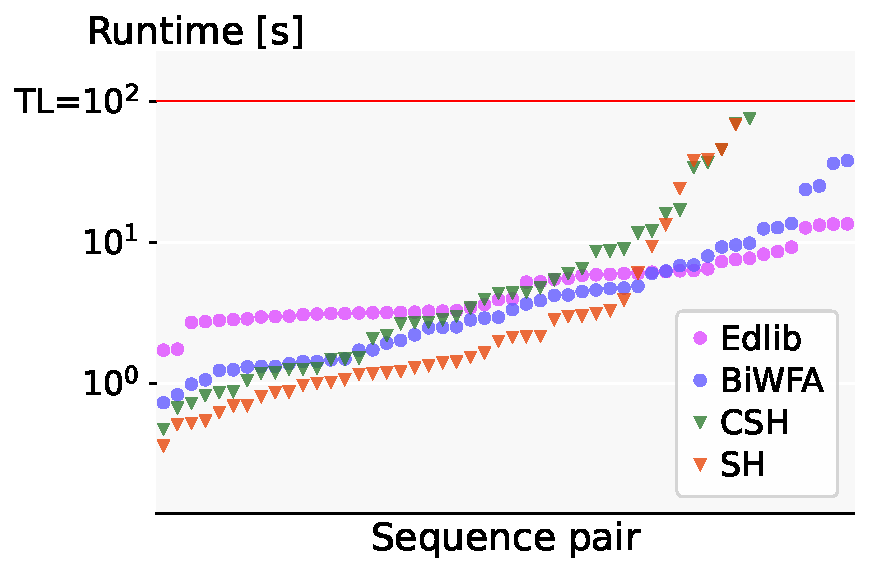
\includegraphics[width=0.48\linewidth]{imgs/fig7/human_sorted_chm13.pdf}}
  \hfill
  \subfloat[NA12878: ONT read errors + biological variation]%
  {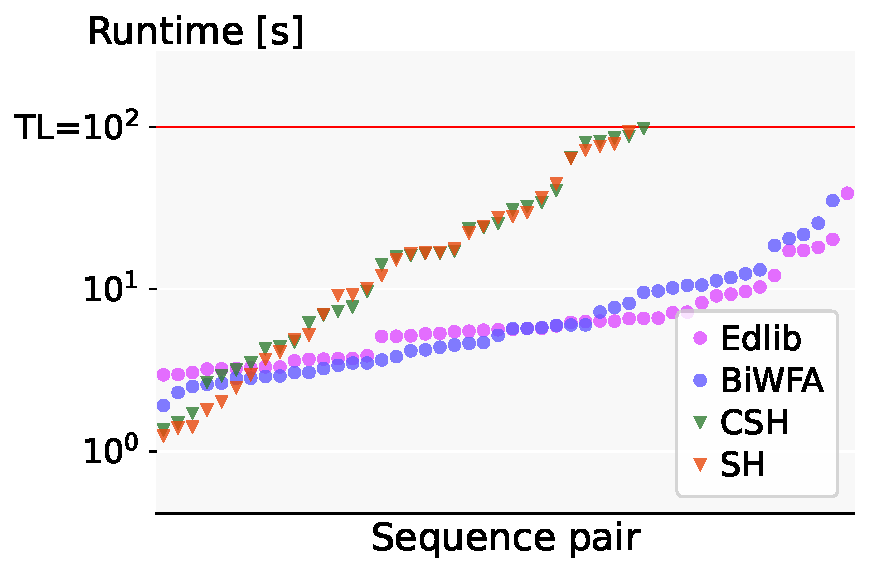
\includegraphics[width=0.48\linewidth]{imgs/fig7/human_sorted_na12878.pdf}}
  \caption[Runtime per sequence (real data)]{Log plot comparison of the
  aligners' runtime on \textbf{real data}. The data points for each individual
  aligner are sorted by alignment time. Alignments that timed out after $100$
  seconds are not shown.}
  \label{GLOBALfig:human-results}
\end{figure}

In this section we compare the exact optimal aligners on long ONT reads from our
human datasets~(\cref{GLOBALfig:human-results}). With the presented minimalistic
features, \astarpa aligns some sequences faster than \wfa and \edlib, but the
high runtime variance makes it slower overall~(\cref{GLOBALsec:variation-human-results}).

% heuristics vs biwfa/edlib
On the dataset without biological variation \datasetOne, \SH is faster than \wfa
and \edlib on $58\%$ of the alignments ($29$ of $50$). On the dataset with
biological variation \datasetTwo, \SH outperforms \wfa and \edlib on $17\%$ of the
alignments ($8$ of $48$) and in other cases is over an order of magnitude
slower. In both datasets, \SH and \CSH time out for the sequences with the
highest edit distances, because they have an error rate larger than the
heuristic can handle efficiently~($e\geq r/k=2/15=13.3\%$).

% SH vs CSH
\CSH usually explores fewer states than \SH since \csh dominates
the \sh. However, in certain cases \CSH is slower than \SH since needs more time
to update the heuristic after pruning (Step 3$'$ in \cref{GLOBALsec:compute-csh}).
%, and %spends up to $98\%$ of its time on this.
